\chapter{Rigs}
\section{General}
There are five rigs in the process control labs.  Each has unique control difficulties.  The following sections will describe how to connect MATLAB to the rigs, how each rig functions and basic procedures to follow.  The procedures described are
\begin{description}
	\item [Commissioning] This procedure is meant to be followed after the rig has been decommissioned at the end of a semester and has been standing for a period without maintenance.  During this operation, constant supervision of the rig is required to ensure that no leaks or other failures occur.
	\item [Wet startup] This procedure is to start the rig after it has been commissioned.
	\item [Shutdown] When the rig is to be used again within the near future, only a shutdown is required.
	\item [Decommissioning] When the rig is to be shelved for a significant period, a full decommissioning should be performed.  This will ensure that no extra fluids or other corrosive materials are left in the equipment and ready the rig for long-term disuse.
\end{description}

\section{The server}
One computer called the \emph{server}\index{server} in the lab is always on and connected to the network.  This computer is running Linux and is very reliable.  Information that is important to the running of the rigs that can not be found in this manual is stored centrally on the server.  Currently the server can be accessed using by navigating to \verb|groa| in windows.  Lab related information, including specific files for each rig, can be found in the directory \verb|lab|.

\section{Matlab control}
Each rig that is to be run from Matlab has a Simulink model associated with it.  These models can be found on the server.  The model will be named to reflect the rig that it represents.  To use this model, copy the model file to the directory where you will be working on the control of the rig.  From the Simulink model browser, you can open the model file and drag the model within onto a worksheet to start controlling the rigs.  These models have been set up to conform to the following standards:
\begin{itemize}\index{rig models!standards}
	\item All final control elements are activated from 0 to 1, in other words from 0\% to 100\%.  
	\item Thermocouples output temperature in \deg Celsius.
	\item Flow meters output flow in units that are specific to the rig, usually to correspond with guages on the rigs.
	\item Level meters output level in mm liquid
\end{itemize}

\section{Acetone}
The acetone flash drum control rig is currently out of commission.
\section{pH Control loop}
\subsection{Overview}
pH control is a notoriously difficult control problem not only due to its highly non-linear nature and large temperature dependence but also due to the extreme conditions experienced by measuring equipment. These problems can be investigated on the rig shown in figure~\ref{fig:rig:ph}.
\begin{figure}
	\centering
	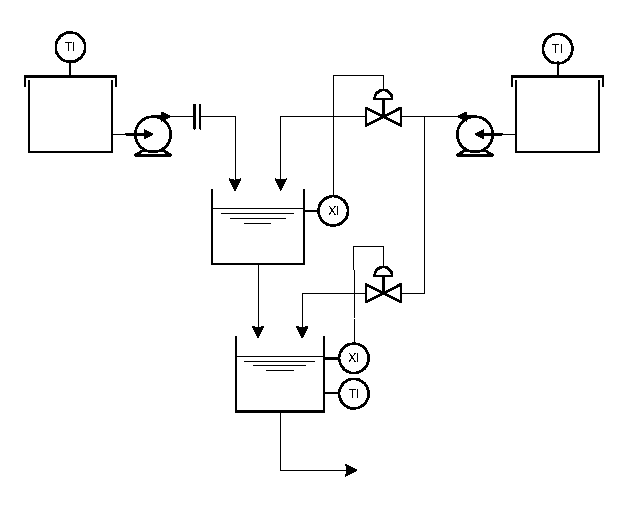
\includegraphics{pH}
	\caption{The pH control rig}
	\label{fig:rig:ph}
\end{figure}
Three temperature measurements are made to provide the possibility for temperature compensation.

\subsection{Procedures}

\subsubsection{Commissioning}

\subsubsection{Startup}

\subsubsection{Shutdown}

\subsubsection{Decommissioning}

\section{Temperature control loop with variable dead time}
The difficulties associated with the control of deadtime processes can be investigated on this rig (shown in figure~\ref{fig:rig:heat}.
\begin{figure}
	\centering
	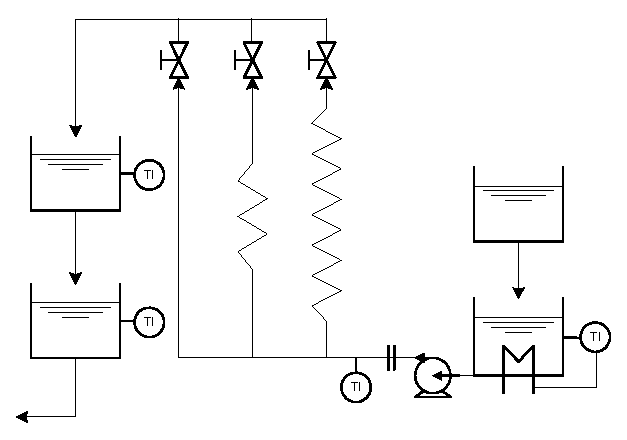
\includegraphics{Heat}
	\caption{The variable dead time temperature control rig}
	\label{fig:rig:heat}
\end{figure}
Three paths with different lengths (and different dead times) can be selected by opening and closing manual valves.  Four temperatures are measured at different points on the control loop and can be controlled by manipulating heat input from an adjustable heating element. 

\subsection{Procedures}
\subsubsection{Commissioning}
\begin{enumerate}
	\item Make a visual inspection of the equipment and ensure that no rust or obstructions are visible on the rig.  Special care should be taken to remove algal growth from the water heater.
	\item Ensure water supply is connected
	\item Ensure drain is open and unconstricted
	\item Ensure that power is supplied to the rig as well as the Thyristor
	\item Open \tagname{HV005} (Water supply valve)
	\item Ensure that water flows into the water heater
	\item Allow water level to stabilise
	\item Ensure that the float activated valve closes
	\item Follow procedure for calibrating thermocouples described in paragraph~\ref{sec:thermocouplecalibration}
\end{enumerate}

\subsubsection{Wet Startup}
This procedure is to start the rig after it has been commissioned.  There must be water in the system and the water supply must be connected with all supply valves open.
\begin{enumerate}
	\item Enable 100\% power on Thyristor
	\item Switch on mixer
	\item Ensure \tagname{HV002}, \tagname{HV003} and \tagname{HV004} are switched to the correct positions for the experiment
	\item Wait for temperature to reach setpoint temperature
	\item Switch on pump
	\item Open \tagname{HV001}
	\item Switch to automatic control on thyristor.
\end{enumerate}

\subsubsection{Shutdown}
This is the standard shutdown when the rig is still to be used in the near future.  It retains water in the rig and keeps it in readiness for a wet startup.
\begin{enumerate}
	\item Stop thyristor by pressing stop button
	\item Stop mixer
	\item Stop pump
	\item Close \tagname{HV001}
\end{enumerate}

\subsubsection{Decommissioning}
\begin{enumerate}
	\item Close \tagname{HV005}
	\item Start pump
	\item Allow tank to drain without allowing the pump to run dry
	\item Stop pump
	\item Allow water to run down from \tagname{T001} (Dead time reservoir tank)
	\item Close \tagname{HV001}
	\item Syphon off remaining water and dry tank
\end{enumerate}
\section{Level and flow control loop}

Interactive level and flow control necessitates the use of multivariable control techniques.  Figure~\ref{fig:rig:levelflow} shows the rig used for this application.  Dead time can be incorporated by using a dead time pan. 
\begin{figure}
	\centering
	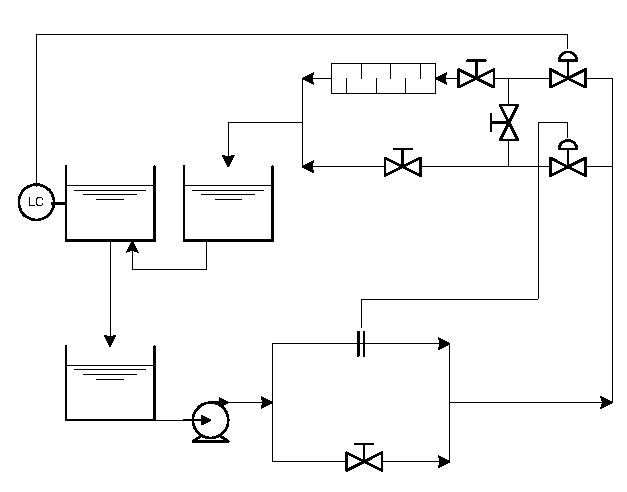
\includegraphics{LevelFlow}
	\caption{The level and flow control loop}
	\label{fig:rig:levelflow}
\end{figure}
The robust nature of the rig makes it ideal for the implementation and development of advanced analysis and control techniques like on-line tuning and fault detection.  Contemporary control techniques such as fuzzy logic or neural network control can also be attempted, as the system dynamics are straightforward and easily checked.

%\subsection{Procedures}

%\subsubsection{Commissioning}

%\subsubsection{Startup}

%\subsubsection{Shutdown}

%\subsubsection{Decommissioning}

\section{Distillation collumn control}
\subsection{Description}
The various control strategies and problems (such as inferential composition measurement) associated with distillation column control can be investigated on the rig shown in figure~\ref{fig:rig:dist}. \begin{figure}
	\centering
	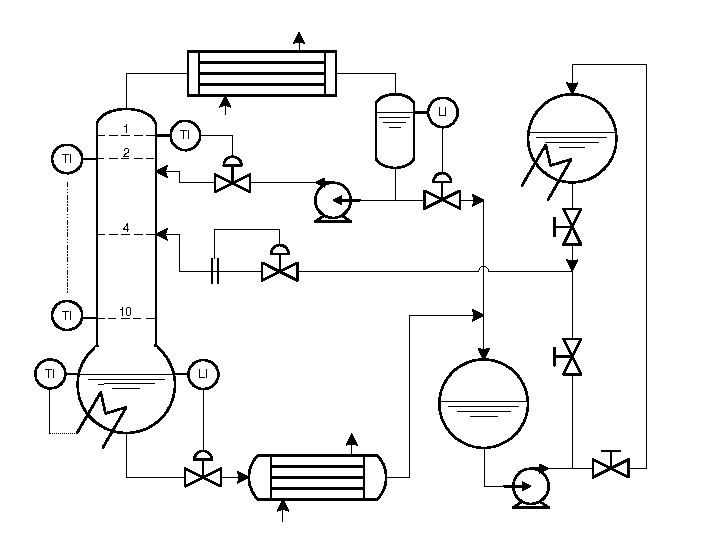
\includegraphics{Dist}
	\caption{The distillation control loop}
	\label{fig:rig:dist}
\end{figure}
Strategies that can be implemented include:
\begin{itemize}
	\item Base layer control system development
	\item Decoupling design and implementation
	\item Constrained model predictive control
	\item Temperature or composition profile control
	\item Non-linear control
	\item Automated start-up and shut down 
\end{itemize}

There are certain control problems unique to this experimental rig. The boiler-accumulator at the bottom of the distillation column is spherical. This makes the level control as well as the boil-up rate highly non-linear. Another control problem identified is that the product is mixed and recycled to the feed drum. This results in output variance being recycled back into the column.

\subsection{Procedures}
\subsubsection{Start-up}
\begin{enumerate}
	\item Open the air supply line.
	\item Adjust the pressure regulator to deliver 200 kPa.
	\item Open \tagname{05HV001} by 10\% (Small fraction).
	\item Set \tagname{05CV002} (feed valve) to 100\%.
	\item Close \tagname{05CV002} when \tagname{05LC001} (Bottoms level) is 80\%.
	\item Switch \tagname{05HS001} (thyristor power) on.
	\item Press the ``Start'' button on the thyristor.
	\item Open the cooling water supply.
	\item Set \tagname{05VC001} (thyristor) to 100\%.
	\item Set \tagname{05VC001} to desired set point when \tagname{05TI001} is more than 60 \deg C.
	\item Switch \tagname{05HS002} on (Reflux pump) when \tagname{05LC002} (Distillate level) is 50\%.
	\item Open \tagname{05CV003} (Reflux) to desired set point.
	\item Set \tagname{05CV002} to the desired set point when \tagname{05TI001} and \tagname{05TI010} stabilises.
	\item Set \tagname{05CV004} (Top) to desired set point.
	\item Set \tagname{05CV005} (Bottom) to desired set point.
\end{enumerate}

\subsubsection{Shut down}
\begin{enumerate}
	\item Close \tagname{05CV002} (Feed)
	\item Close \tagname{05CV004} (Top)
	\item Close \tagname{05CV005} (Bottom)
	\item Switch \tagname{05HS002} off (Reflux pump)
	\item Close \tagname{05CV003} (Reflux valve)
	\item Set \tagname{05VC001} (Thyristor) to 0\%
	\item Switch \tagname{05HS001} off (Thyristor power)
	\item Close the air supply line
	\item Close \tagname{05HV001} when the air pressure is zero
	\item Close the cooling water when \tagname{05TI001} is less than 60 \deg C
\end{enumerate}
